
 \documentclass[11pt,twocolumn]{article}

\usepackage{pslatex}
\usepackage{fullpage}
\usepackage{alltt}
\usepackage{rotating}
\usepackage{float}
\usepackage{pifont}
\usepackage{wasysym}
\usepackage{verbatim} 

\usepackage{listings}
\usepackage{url}
\usepackage{color}
\usepackage{makeidx}
\usepackage{textcomp}
\setcounter{section}{0}
\usepackage{eso-pic}
\usepackage{cite}
\usepackage{type1cm}
\usepackage{multirow}
\usepackage[table]{xcolor}
\usepackage{booktabs, multicol, multirow}
\usepackage{balance}
\usepackage{booktabs}
\usepackage{bigstrut}


\lstset{
    language=Python,
    basicstyle=\ttfamily\fontsize{3.5mm}{0.9xem}\selectfont,
    breaklines=true,
    prebreak=\raisebox{0ex}[0ex][0ex]{\ensuremath{\hookleftarrow}},
    frame=l,
    showtabs=false,
    showspaces=false,
    showstringspaces=false,
    keywordstyle=\bfseries,
    emph={bootstrap,a12,DivideonEntropy,discretize,furthest,FASTMAP,CrossTree,project,WHERE4,score,cart,model}, emphstyle=\bfseries\color{blue},
    stringstyle=\color{green!50!black},
    commentstyle=\color{gray}\itshape,
    numbers=left,
    captionpos=t,
    escapeinside={\%*}{*)}
}

\newcommand{\captionfonts}{\sffamily\scriptsize}
\lstset{%
   basicstyle=\scriptsize\tt,%numbers=left,%   numberstyle=\tiny,% stepnumber=2,%%
   upquote=true,%
   framexleftmargin=1mm, frame=shadowbox, rulesepcolor=\color{black}}
\newcommand{\codelist}[2]{\begin{figure}[h]%
            \index{files!#1}
           	\lstinputlisting{#2}
           	\caption{CODE: {\tt #1}}%
            \label{fig:#1}\end{figure}}
            
\newcommand{\pseudocode}[2]{\begin{figure}[h]%
            \index{files!#1}
           	\lstinputlisting{#2}
           	\caption{Pseudocode: {\tt #1}}%
            \label{fig:#1}\end{figure}}            


%quarts
\usepackage{colortbl} % not sure if needed
\usepackage[table]{xcolor} % not sure if needed

%%%% needed %%%
\usepackage{picture}
\newcommand{\quart}[3]{\begin{picture}(100,6)%1
{\color{black}\put(#3,3){\circle*{4}}\put(#1,3){\line(1,0){#2}}}\end{picture}}


\begin{document}
\thispagestyle{empty}



\begin{figure}[!b]
\begin{center}
\begin{lstlisting}[mathescape,frame=l,numbers=left]
def FASTMAP(Sn): 
  "Project data on a line between 
   two distant points"
  z          = random.choose(Sn)
  east       = furthest(z, Sn)
  west       = furthest(east, Sn)
  Sn.poles = (west,east)
  c          = dist(west,east)     
  for one in Sn.members: 
    one.X,one.Y = project(west,east,c,one)
  return Sn #data members updated with (X,Y)

def project(west, east, c, x): 
  "Project x onto line east to west"
  a = dist(x,west)
  b = dist(x,east)
  X = (a*a + c*c - b*b)/(2*c), # cosine rule
  Y = (a*a - X)**0.5 # dist to line b/w poles
  return X,Y
         
def furthest(x,Sn): # furthest from x?
  out, max = x,0
  for y in Sn:
    d = dist(x,y)
    if d > max: out, max = y, d
  return out

\end{lstlisting}
\end{center}
\caption{Splitting data with FASTMAP}
\label{fig:FASTMAP}   
\end{figure}


\begin{figure}[!b]
\begin{center}
\begin{lstlisting}[mathescape,frame=l,numbers=left]
def WHERE4(Sn,min,max):
  "Recursive cluster quadrants of data"
  if Sn.length > min: 
    if Sn.length < max:
      yield Sn
    else:
      Xcap,Ycap = mean(Sn.Xs,Sn.Ys)
      for one in Sn:
        Sll += one if one.X < Xcap 
                      and one.Y < Ycap
        Slh += one if one.X < Xcap 
                      and one.Y > Ycap
        Shl += one if one.X > Xcap 
                      and one.Y < Ycap
        Shh += one if one.X > Xcap 
                      and one.Y > Ycap
      for S in (Sll,Slh,Shl,Shh): 
        WHERE4(S,min,max)
  else:
    yield Sn
\end{lstlisting}
\end{center}
\caption{Recursing Spectrally in quadrants using WHERE4 Algorithm}
\label{fig:WHERE4}   
\end{figure}


\begin{figure}[!b]
\begin{center}
\begin{lstlisting}[mathescape,frame=l,numbers=left]
def CrossTree(Sn):
  "Tree of clusters and results 
   from their differences"
  
  #Calculate (X,Y) of solutions
  Sn = FASTMAP(Sn)   
  #Accumulate Clusters
  Cm = [C for C in WHERE4(Sn,min,max)]   
  #Replace data with discretized values
  Cm = Discretize(Cm)
  #Score clusters
  BetterC,WorseC = score(Cm)  
  
  #Build CART Decision Tree
  Dtree = cart(Cm)
  
  #Prune same and more leaves
  for leaf in Dtree:
    if size(leaf.clusters) > 1: 
      Dtree.prune(leaf)  
  for subtree in Dtree:
    if size(subtree.uniq_clusters) < 2:
      Dtree.prune(subtree)

  for Branch in Dtree: 

    #Find a better branch for current branch
    BBranch = Dtree.nearest_best(Branch.C,  
                                 BetterC)   

    if BBranch:
      #Contrast Set(CS) represents diff b/w
      #limits of Better and Worse Cluster
      CS = Dtree.differ(WBranch.C,
                        BBranch.C)
    
      #Generate new population from model 
      #using Contrast set
      ContrastSn = model(Size=Branch.C.size*10,
                         ContrastSet)

      q1,q2,q3,q4 += ContrastSn.qs
    
    else:
      #Balance distribution
      q1,q2,q3,q4 += Limits(Branch.C).qs

  #25\%,median,75\%,Maximum
  return q1,q2,q3,q4

\end{lstlisting}
\end{center}
\caption{Generating Deltas between clusters using CrossTree}
\label{fig:CrossTree}   
\end{figure}


\begin{figure}[!b]
\begin{center}
\begin{lstlisting}[mathescape,frame=l,numbers=left]
def score(Cm):
  "Divides set of clusters into better 
   and worse based on objectives"
   better,worse,similar = 0,0,0
   for this in Cm:
     for other in Cm:
       for obj in Cm.objectives:
         pop1,pop2 = this.pop[obj],
                     other.pop[obj]
         #similar check
         if a12(pop1,pop2) and 
            bootstrap(pop1,pop2): 
           similar += 1
         #different being better or worse
         elif median(pop1) > median(pop2):
           better += 1
         else:
           worse += 1
       if better > 0 and worse == 0:
         scores[this] += 1
   #top square root of len are better
   Cm,cut = sorted(scores),scores.len**0.5
   return Cm[:cut],Cm[cut:] 
\end{lstlisting}
\end{center}
\caption{Generating Deltas between clusters using CrossTree}
\label{fig:discretize}   
\end{figure}


\begin{figure}[!b]
\begin{center}
\begin{lstlisting}[mathescape,frame=l,numbers=left]
def discretize(Cm):
  "Discretizes data into bin and replaces 
   its values with respective bin ids"
   #find best cut with least entropy 
   #to predict clusters
   for C in Cm:
     pairs[d].append(C.id,C.dvalue)
   for d in decisions:
     bins[d] = divide(pairs[d])

   def divide(this):
     lhs,rhs   = Counts(),
                 Counts(sym(x) for x in this)
     for j,x  in enumerate(this): 
       maybe= lhs.n/n0*lhs.ent()  
              + rhs.n/n0*rhs.ent()
       if maybe < least:
         cut,least = j,maybe
       rhs - sym(x)
       lhs + sym(x)
     if cut:
       return bins+=divide(this[:cut])
                  +=divide(this[cut:])
     else: return bins

   for C,d in Cm,Cm.decisions:
     C.values[d] = bins.id(C,d)

   return Cm
\end{lstlisting}
\end{center}
\caption{Generating Deltas between clusters using CrossTree}
\label{fig:crosstrees}   
\end{figure}


\begin{figure}
\begin{center}
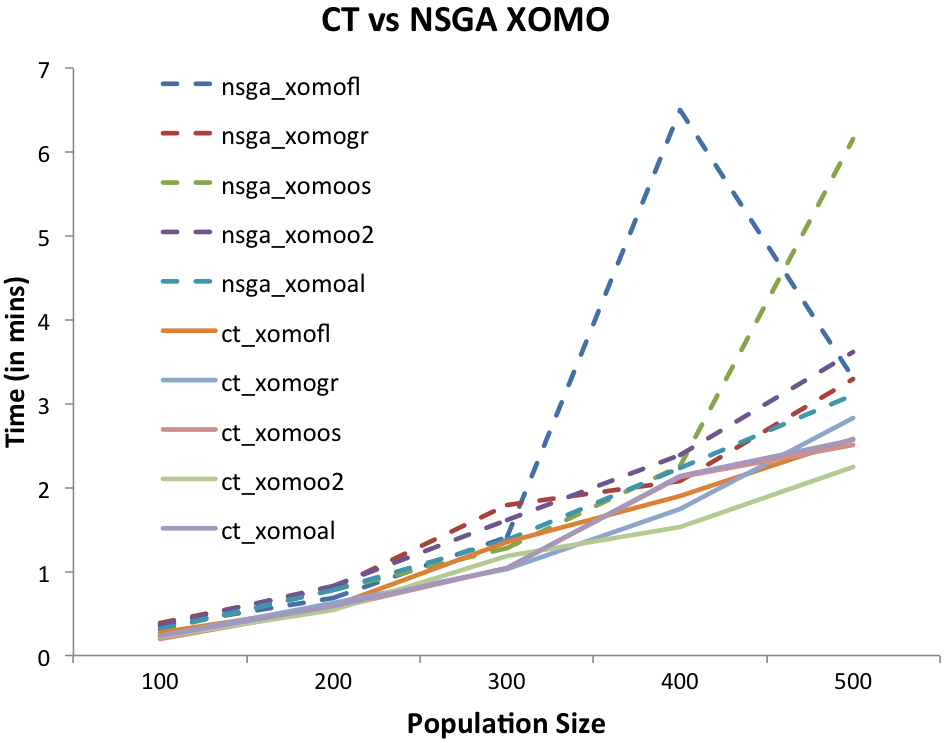
\includegraphics[width=8cm]{figures/xomotimes.png}
\end{center}
\caption[CT vs. NSGA II XOMO]{ Times for CT and NSGA II on XOMO Model.}
\label{fig:xomotimes}
\end{figure}


\begin{figure}
\begin{center}
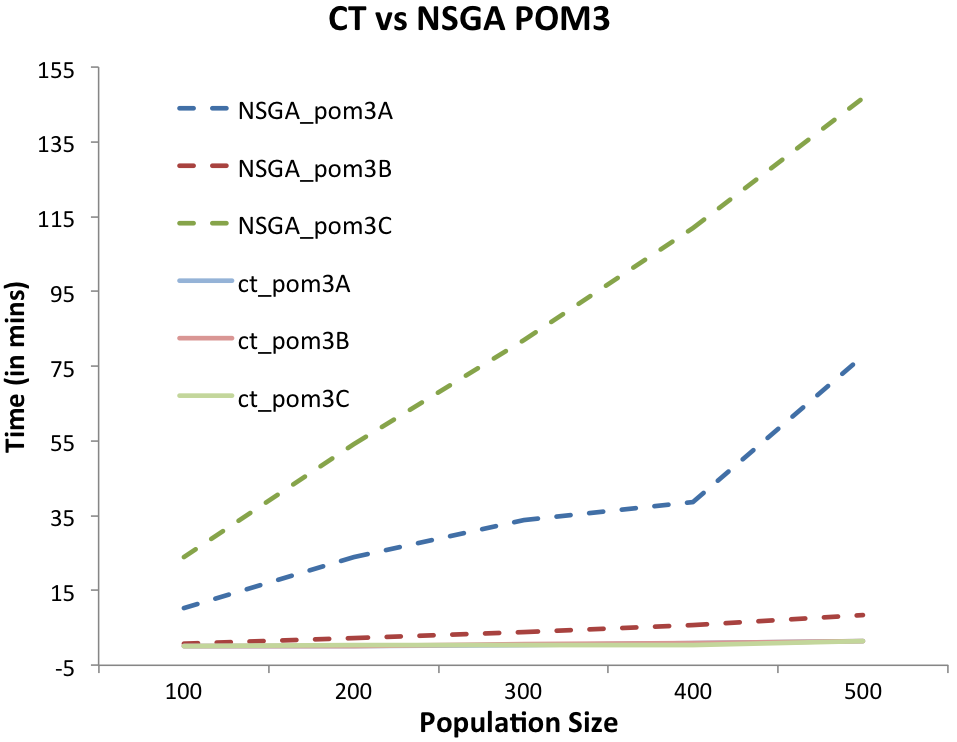
\includegraphics[width=8cm]{figures/pomtimes.png}
\end{center}
\caption[CT vs. NSGA II POM]{ Times for CT and NSGA II on POM Model.}
\label{fig:pomtimes}
\end{figure}


\begin{figure}
\begin{center}
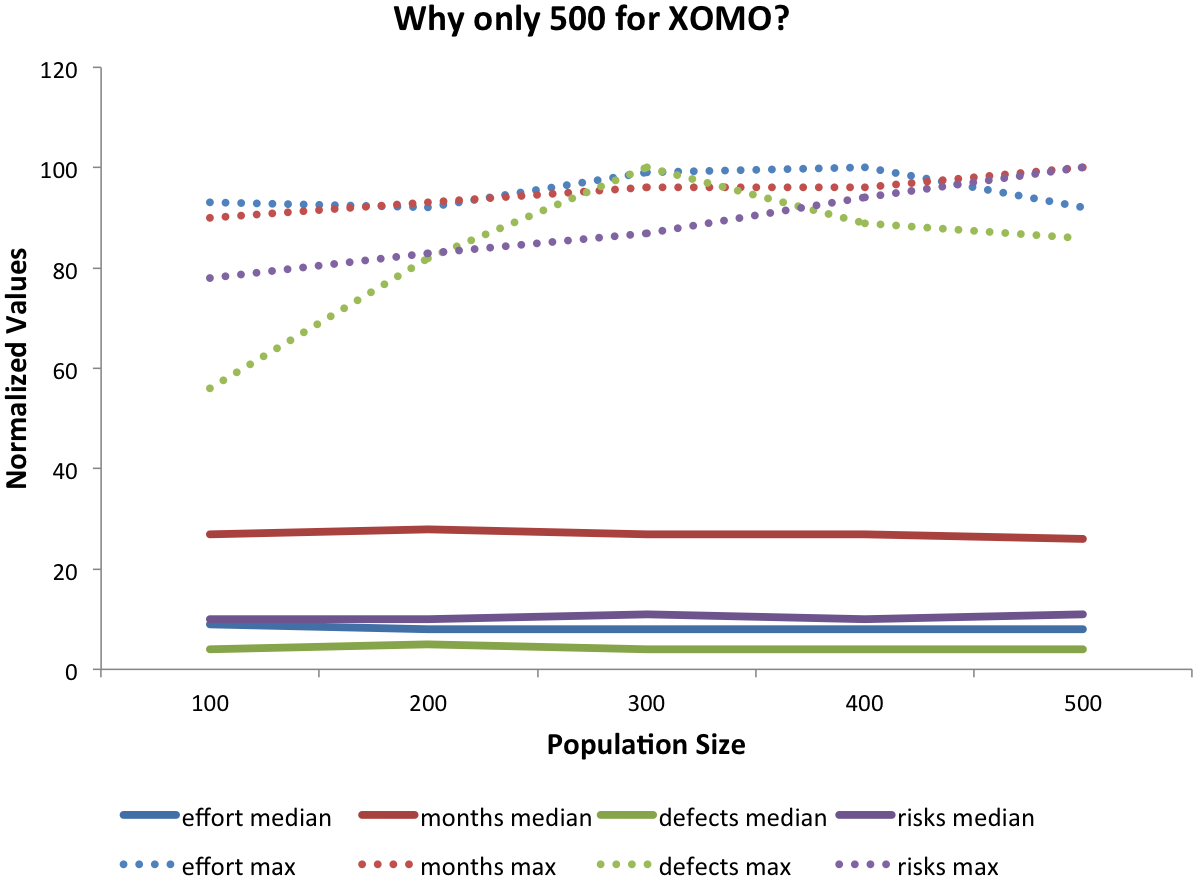
\includegraphics[width=8cm]{figures/why500xomo.png}
\end{center}
\caption[Why 500 xomo?]{ Median and Max of NSGA on XOMO when population size increases from 100 to 500.}
\label{fig:why500xomo}
\end{figure}

\begin{figure}
\begin{center}
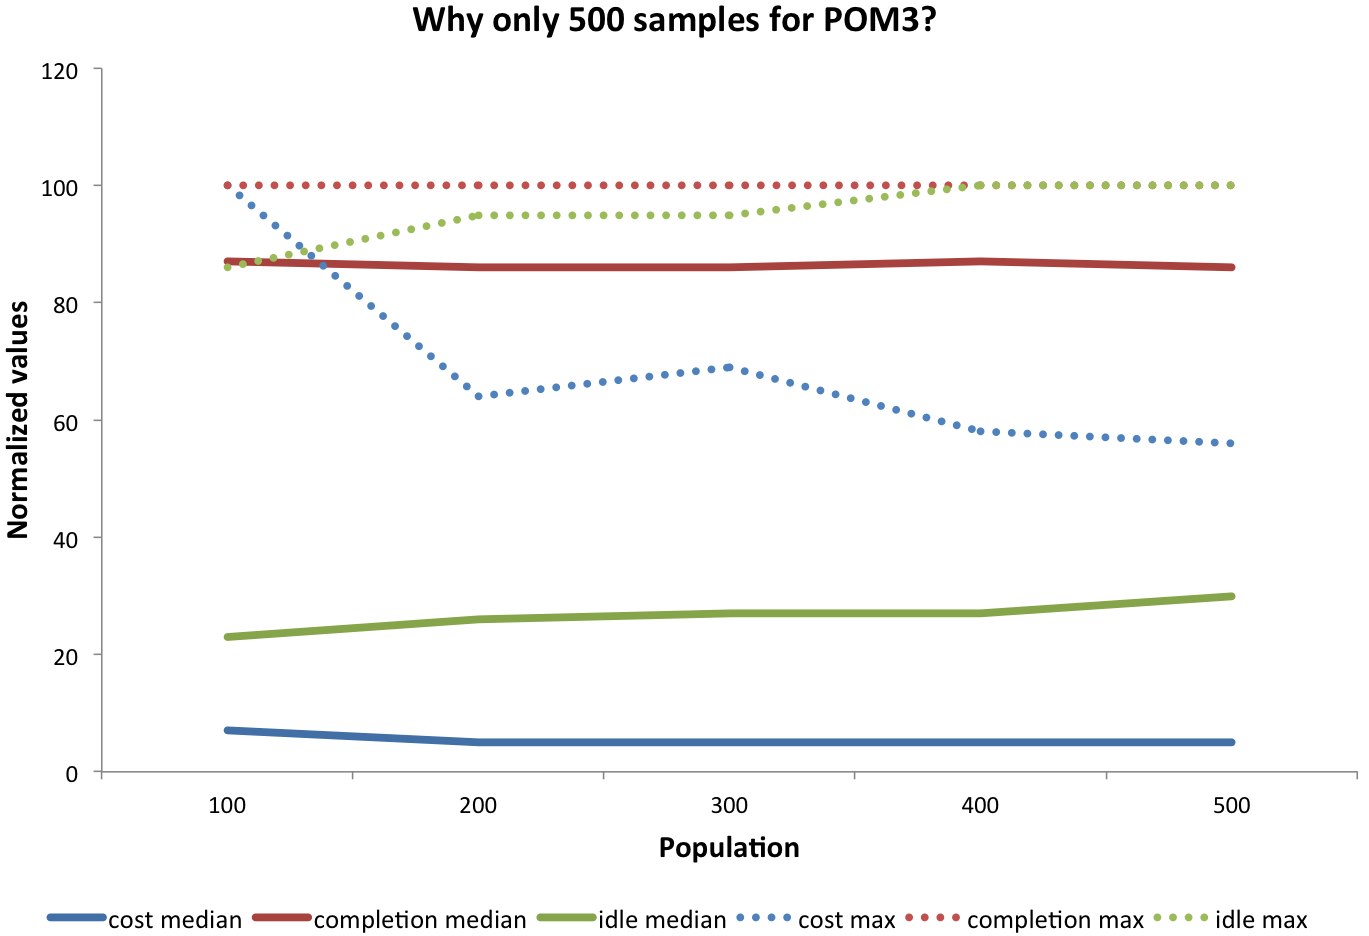
\includegraphics[width=8cm]{figures/why500pom.png}
\end{center}
\caption[Why 500 pom?]{ Median and Max of NSGA on POM when population size increases from 100 to 500.}
\label{fig:why500pom}
\end{figure}




\begin{figure}[!t]

{\scriptsize
{\bf Model: POM3A}

{\scriptsize \begin{tabular}{l@{~~~}l@{~~~}l@{~~~}r@{~~~}r@{~~~}c}
\arrayrulecolor{darkgray}
\rowcolor[gray]{.7}  Objective & method & median & IQR & \\ 
\rowcolor[gray]{.9} cost  & Base Line & 32 & 28 & \quart{19.0}{28.0}{32.0} \\ 
 & CT0 & 35 & 25 & \quart{23.0}{25.0}{35.0} \\ 
 & NSGA II & 3 & 0 & \quart{3.0}{0.0}{3.0} \\ 
\rowcolor[gray]{.9} completion  & Base Line & 85 & 2 & \quart{74.0}{2.0}{85.0} \\ 
 & CT0 & 75 & 0 & \quart{65.0}{0.0}{75.0} \\ 
 & NSGA II & 86 & 1 & \quart{78.0}{1.0}{86.0} \\ 
\rowcolor[gray]{.9} idle  & Base Line & 22 & 36 & \quart{1.0}{36.0}{22.0} \\ 
 & CT0 & 17 & 29 & \quart{0.0}{29.0}{17.0} \\ 
 & NSGA II & 31 & 45 & \quart{4.0}{45.0}{31.0} \\ 
\end{tabular}}

}
{\scriptsize
{\bf Model: POM3B}

{\scriptsize \begin{tabular}{l@{~~~}l@{~~~}l@{~~~}r@{~~~}r@{~~~}c}
\arrayrulecolor{darkgray}
\rowcolor[gray]{.7}  Objective & method & median & IQR & \\ 
\rowcolor[gray]{.9} cost  & Base Line & 32 & 27 & \quart{20.0}{27.0}{32.0} \\ 
 & CT0 & 19 & 14 & \quart{12.0}{14.0}{19.0} \\ 
 & NSGA II & 6 & 0 & \quart{5.0}{0.0}{6.0} \\ 
\rowcolor[gray]{.9} completion  & Base Line & 84 & 2 & \quart{74.0}{2.0}{84.0} \\ 
 & CT0 & 55 & 0 & \quart{47.0}{0.0}{55.0} \\ 
 & NSGA II & 86 & 2 & \quart{77.0}{2.0}{86.0} \\ 
\rowcolor[gray]{.9} idle  & Base Line & 29 & 37 & \quart{5.0}{37.0}{29.0} \\ 
 & CT0 & 17 & 27 & \quart{0.0}{27.0}{17.0} \\ 
 & NSGA II & 32 & 47 & \quart{6.0}{47.0}{32.0} \\ 
\end{tabular}}

}

{\scriptsize
{\bf Model: POM3C}

{\scriptsize \begin{tabular}{l@{~~~}l@{~~~}l@{~~~}r@{~~~}r@{~~~}c}
\arrayrulecolor{darkgray}
\rowcolor[gray]{.7}  Objective & method & median & IQR & \\ 
\rowcolor[gray]{.9} cost  & Base Line & 40 & 25 & \quart{27.0}{25.0}{40.0} \\ 
 & CT0 & 31 & 20 & \quart{20.0}{20.0}{31.0} \\ 
 & NSGA II & 10 & 0 & \quart{8.0}{0.0}{10.0} \\ 
\rowcolor[gray]{.9} completion  & Base Line & 90 & 0 & \quart{82.0}{0.0}{90.0} \\ 
 & CT0 & 63 & 1 & \quart{54.0}{1.0}{63.0} \\ 
 & NSGA II & 90 & 1 & \quart{83.0}{1.0}{90.0} \\ 
\rowcolor[gray]{.9} idle  & Base Line & 34 & 33 & \quart{8.0}{33.0}{34.0} \\ 
 & CT0 & 21 & 25 & \quart{0.0}{25.0}{21.0} \\ 
 & NSGA II & 36 & 41 & \quart{8.0}{41.0}{36.0} \\ 
\end{tabular}}

}
\caption{Model: POM3}\label{fig:pom3}
\end{figure}




\begin{figure}[!t]

{\scriptsize
{\bf Model: XOMOAL}

{\scriptsize \begin{tabular}{l@{~~~}l@{~~~}l@{~~~}r@{~~~}r@{~~~}c}
\arrayrulecolor{darkgray}
\rowcolor[gray]{.7}  Objective & method & median & IQR & \\ 
\rowcolor[gray]{.9} effort  & Base Line & 6 & 3 & \quart{1.0}{3.0}{6.0} \\ 
 & CT0 & 4 & 4 & \quart{0.0}{4.0}{4.0} \\ 
 & NSGA II & 11 & 12 & \quart{3.0}{12.0}{11.0} \\ 
\rowcolor[gray]{.9} months  & Base Line & 20 & 0 & \quart{16.0}{0.0}{20.0} \\ 
 & CT0 & 19 & 4 & \quart{14.0}{4.0}{19.0} \\ 
 & NSGA II & 36 & 14 & \quart{27.0}{14.0}{36.0} \\ 
\rowcolor[gray]{.9} defects  & Base Line & 14 & 22 & \quart{5.0}{22.0}{14.0} \\ 
 & CT0 & 3 & 6 & \quart{1.0}{6.0}{3.0} \\ 
 & NSGA II & 3 & 5 & \quart{0.0}{5.0}{3.0} \\ 
\rowcolor[gray]{.9} risks  & Base Line & 73 & 17 & \quart{64.0}{17.0}{73.0} \\ 
 & CT0 & 7 & 6 & \quart{4.0}{6.0}{7.0} \\ 
 & NSGA II & 5 & 8 & \quart{0.0}{8.0}{5.0} \\ 
\end{tabular}}

}

{\scriptsize
{\bf Model: XOMOFL}

{\scriptsize \begin{tabular}{l@{~~~}l@{~~~}l@{~~~}r@{~~~}r@{~~~}c}
\arrayrulecolor{darkgray}
\rowcolor[gray]{.7}  Objective & method & median & IQR & \\ 
\rowcolor[gray]{.9} effort  & Base Line & 19 & 15 & \quart{8.0}{15.0}{19.0} \\ 
 & CT0 & 4 & 5 & \quart{0.0}{5.0}{4.0} \\ 
 & NSGA II & 11 & 12 & \quart{4.0}{12.0}{11.0} \\ 
\rowcolor[gray]{.9} months  & Base Line & 27 & 1 & \quart{20.0}{1.0}{27.0} \\ 
 & CT0 & 19 & 0 & \quart{15.0}{0.0}{19.0} \\ 
 & NSGA II & 36 & 13 & \quart{27.0}{13.0}{36.0} \\ 
\rowcolor[gray]{.9} defects  & Base Line & 22 & 29 & \quart{10.0}{29.0}{22.0} \\ 
 & CT0 & 2 & 3 & \quart{0.0}{3.0}{2.0} \\ 
 & NSGA II & 5 & 7 & \quart{1.0}{7.0}{5.0} \\ 
\rowcolor[gray]{.9} risks  & Base Line & 87 & 5 & \quart{82.0}{5.0}{87.0} \\ 
 & CT0 & 2 & 0 & \quart{0.0}{0.0}{2.0} \\ 
 & NSGA II & 6 & 9 & \quart{1.0}{9.0}{6.0} \\ 
\end{tabular}}

}

{\scriptsize
{\bf Model: XOMOGR}

{\scriptsize \begin{tabular}{l@{~~~}l@{~~~}l@{~~~}r@{~~~}r@{~~~}c}
\arrayrulecolor{darkgray}
\rowcolor[gray]{.7}  Objective & method & median & IQR & \\ 
\rowcolor[gray]{.9} effort  & Base Line & 7 & 5 & \quart{3.0}{5.0}{7.0} \\ 
 & CT0 & 3 & 3 & \quart{0.0}{3.0}{3.0} \\ 
 & NSGA II & 13 & 14 & \quart{6.0}{14.0}{13.0} \\ 
\rowcolor[gray]{.9} months  & Base Line & 21 & 0 & \quart{17.0}{0.0}{21.0} \\ 
 & CT0 & 23 & 2 & \quart{18.0}{2.0}{23.0} \\ 
 & NSGA II & 39 & 16 & \quart{29.0}{16.0}{39.0} \\ 
\rowcolor[gray]{.9} defects  & Base Line & 16 & 22 & \quart{7.0}{22.0}{16.0} \\ 
 & CT0 & 1 & 2 & \quart{0.0}{2.0}{1.0} \\ 
 & NSGA II & 4 & 5 & \quart{1.0}{5.0}{4.0} \\ 
\rowcolor[gray]{.9} risks  & Base Line & 74 & 13 & \quart{66.0}{13.0}{74.0} \\ 
 & CT0 & 6 & 3 & \quart{3.0}{3.0}{6.0} \\ 
 & NSGA II & 5 & 8 & \quart{0.0}{8.0}{5.0} \\ 
\end{tabular}}

}
\caption{Model: XOMO}\label{fig:xomo1}
\end{figure}

\begin{figure}[!t]

{\scriptsize
{\bf Model: XOMOO2}

{\scriptsize \begin{tabular}{l@{~~~}l@{~~~}l@{~~~}r@{~~~}r@{~~~}c}
\arrayrulecolor{darkgray}
\rowcolor[gray]{.7}  Objective & method & median & IQR & \\ 
\rowcolor[gray]{.9} effort  & Base Line & 5 & 0 & \quart{3.0}{0.0}{5.0} \\ 
 & CT0 & 7 & 1 & \quart{6.0}{1.0}{7.0} \\ 
 & NSGA II & 13 & 14 & \quart{6.0}{14.0}{13.0} \\ 
\rowcolor[gray]{.9} months  & Base Line & 25 & 0 & \quart{23.0}{0.0}{25.0} \\ 
 & CT0 & 20 & 0 & \quart{19.0}{0.0}{20.0} \\ 
 & NSGA II & 43 & 20 & \quart{33.0}{20.0}{43.0} \\ 
\rowcolor[gray]{.9} defects  & Base Line & 37 & 24 & \quart{25.0}{24.0}{37.0} \\ 
 & CT0 & 1 & 0 & \quart{1.0}{0.0}{1.0} \\ 
 & NSGA II & 5 & 8 & \quart{1.0}{8.0}{5.0} \\ 
\rowcolor[gray]{.9} risks  & Base Line & 79 & 16 & \quart{67.0}{16.0}{79.0} \\ 
 & CT0 & 13 & 0 & \quart{12.0}{0.0}{13.0} \\ 
 & NSGA II & 6 & 10 & \quart{0.0}{10.0}{6.0} \\ 
\end{tabular}}

}
{\scriptsize
{\bf Model: XOMOOS}

{\scriptsize \begin{tabular}{l@{~~~}l@{~~~}l@{~~~}r@{~~~}r@{~~~}c}
\arrayrulecolor{darkgray}
\rowcolor[gray]{.7}  Objective & method & median & IQR & \\ 
\rowcolor[gray]{.9} effort  & Base Line & 3 & 0 & \quart{2.0}{0.0}{3.0} \\ 
 & CT0 & 8 & 2 & \quart{6.0}{2.0}{8.0} \\ 
 & NSGA II & 13 & 15 & \quart{6.0}{15.0}{13.0} \\ 
\rowcolor[gray]{.9} months  & Base Line & 19 & 0 & \quart{18.0}{0.0}{19.0} \\ 
 & CT0 & 24 & 2 & \quart{22.0}{2.0}{24.0} \\ 
 & NSGA II & 41 & 19 & \quart{31.0}{19.0}{41.0} \\ 
\rowcolor[gray]{.9} defects  & Base Line & 7 & 4 & \quart{4.0}{4.0}{7.0} \\ 
 & CT0 & 1 & 1 & \quart{0.0}{1.0}{1.0} \\ 
 & NSGA II & 5 & 9 & \quart{1.0}{9.0}{5.0} \\ 
\rowcolor[gray]{.9} risks  & Base Line & 90 & 4 & \quart{85.0}{4.0}{90.0} \\ 
 & CT0 & 20 & 14 & \quart{9.0}{14.0}{20.0} \\ 
 & NSGA II & 8 & 13 & \quart{0.0}{13.0}{8.0} \\ 
\end{tabular}}

}
\caption{Model: XOMO}\label{fig:xomo}
\end{figure}


\begin{figure}[!t]

{\scriptsize
{\bf Model: POM3}
{\scriptsize \begin{tabular}{l@{~~~}c@{~~~}c@{~~~}c@{~~~}c@{~~~}c}
\arrayrulecolor{darkgray}
\rowcolor[gray]{.7}  Model & Value & Cost & Completion & Idle \\ 
pom3A & 0 & 30.76 & 0.12 & 0.04  \\
pom3B & 0 & 575.69 & 0.12 & 0.03  \\
pom3C & 0 & 83.5 & 0.1 & 0.08  \\
pom3A & 100 & 1933.55 & 1.0 & 0.82  \\
pom3B & 100 & 21916.18 & 1.0 & 0.81  \\
pom3C & 100 & 1830.55 & 1.0 & 0.69  \\ 
\end{tabular}}
}

{\scriptsize
{\bf Model: XOMO}
{\scriptsize \begin{tabular}{l@{~~~}c@{~~~}c@{~~~}c@{~~~}c@{~~~}c@{~~~}c}
\arrayrulecolor{darkgray}
\rowcolor[gray]{.7} Model & Value & Effort & Months & Defects & Risks \\ 
xomoal & 0 & 343.25 & 5.05 & 2298.1 & 0.69  \\
xomofl & 0 & 314.32 & 5.76 & 1180.89 & 0.55  \\
xomogr & 0 & 207.79 & 4.52 & 969.14 & 0.72  \\
xomoo2 & 0 & 179.9 & 1.67 & 1204.4 & 0.66  \\
xomoos & 0 & 120.06 & 1.67 & 1711.01 & 0.66  \\
xomoal & 100 & 6302.63 & 68.98 & 103503.64 & 22.55  \\
xomofl & 100 & 6243.79 & 67.54 & 83713.17 & 20.78  \\
xomogr & 100 & 6177.7 & 65.31 & 114610.14 & 20.41  \\
xomoo2 & 100 & 6290.36 & 63.86 & 74828.94 & 18.52  \\
xomoos & 100 & 6739.59 & 66.83 & 64776.58 & 13.55  \\ 
\end{tabular}}
}
\caption{XOMO and POM3 0100 values}\label{fig:xomopom100}
\end{figure}


\end{document}

